\chapter{Introduction}
% \setlength\epigraphrule{0pt}
\epigraph{ 
Aspetti, signorina,\\
le dir\`{o} con due parole\\
chi son, e che faccio, \\
come vivo.  Vuole?%\footnote{Wait, mademoiselle,\backslash I shall tell you with two words \backslash who I am, what I do, \backslash and how I live.  May I?}
}{Rodolfo introduces himself to Mimi in the first act of \textit{La Boheme} by Giacomo Puccini (1858--1924).}

In this chapter I provide what I hope is an adequate description of the key concepts related to the research tackled in this thesis, in addition to the necessary technical background.
While I touch on the overall motivation for my research along the way (specially in Section~\ref{sec:goals}), the specific characterisation of the problems investigated is left to the Introduction/Background section in each chapter. 

\section{Viral phylodynamics}

RNA viruses (e.g. HIV, Influenza, MERS-CoV, Ebola virus) are amongst the leading causes of morbidity and mortality in humans and livestock~\citep{Woolhouse2002}.
The combination of high mutation rates and low generation times means that these pathogens evolve at a time scale such that their genomes can be used to detect the effects of epidemiological and ecological events~\citep{Drummond2003,Grenfell2004,Duffy2008,Pybus2009}.
The recent years have witnessed an unprecedented increase in the availability of molecular sequences from several organisms, specially from fast-evolving RNA viruses~\citep{Benson2014}.
This growth in the availability and quality of data has in turn made it possible to expand the repertoire of scientific questions that can be asked: what factors drive virus emergence within and transmission between populations~\citep{Dudas2017,Dudas2018}? How do population dynamics shape viral circulation patterns~\citep{Volz2013,Bedford2015}?

To tackle these questions it is necessary to bridge the fields of evolutionary biology and epidemiology on what is now known as ``viral phylodynamics''~\citep{Grenfell2004,Volz2013,Pybus2013}.
One commonly accepted definition of phylodynamics states that phylodynamics is concerned with the ``study of how epidemiological, immunological, and evolutionary processes act and potentially interact to shape viral phylogenies''~\citep{Grenfell2004}.
As a theoretical framework, phylodynamics couples coalescent theory and mathematical modelling to understand how population or epidemic dynamics map onto phylogenies, and how to incorporate data from several sources into a coherent inference framework~\citep{Kuhnert2011}.
However, as argued by~\cite{Hall2015} (Chapter 1, page 2), phylodynamics can also be understood as employing phylogenetic methods to obtain estimates of the ancestry between pathogen isolates and the timing of the lineage-splitting events, and then using this information to inform epidemiological inference, an approach called ``phylogenetic epidemiology'' by~\cite{Kuhnert2011}.

Another instance of phylogenetic models being used to inform epidemiological inference without reference to a unified theoretical framework is the estimation of past population dynamics using coalescent methods (see below) which are then compared with epidemiological time series in order to gain epidemiological insight (see Figure 3 in~\cite{Bennett2009} for  an example).
Figure~\ref{fig:timetree} is meant to illustrate one of the end products of a phylodynamic analysis using BEAST~\citep{Drummond2007,Drummond2012}, with a time-calibrated phylogeny built using sequences from a fast-evolving RNA virus (Dengue virus serotype 2).
A \textbf{time-calibrated phylogeny} is a rooted tree in which the branch lengths are measured in units of calendar time (see Appendix A for a thorough description).
The conjunction of time calibration and relaxed clocks allows us to estimate the age of the common ancestor of the circulating strains, as well as identify lineages that evolve faster than others.
In an epidemiological context, such information may prove extremely useful when designing strategies to mitigate disease transmission.

\begin{figure}[!ht]
\begin{center}
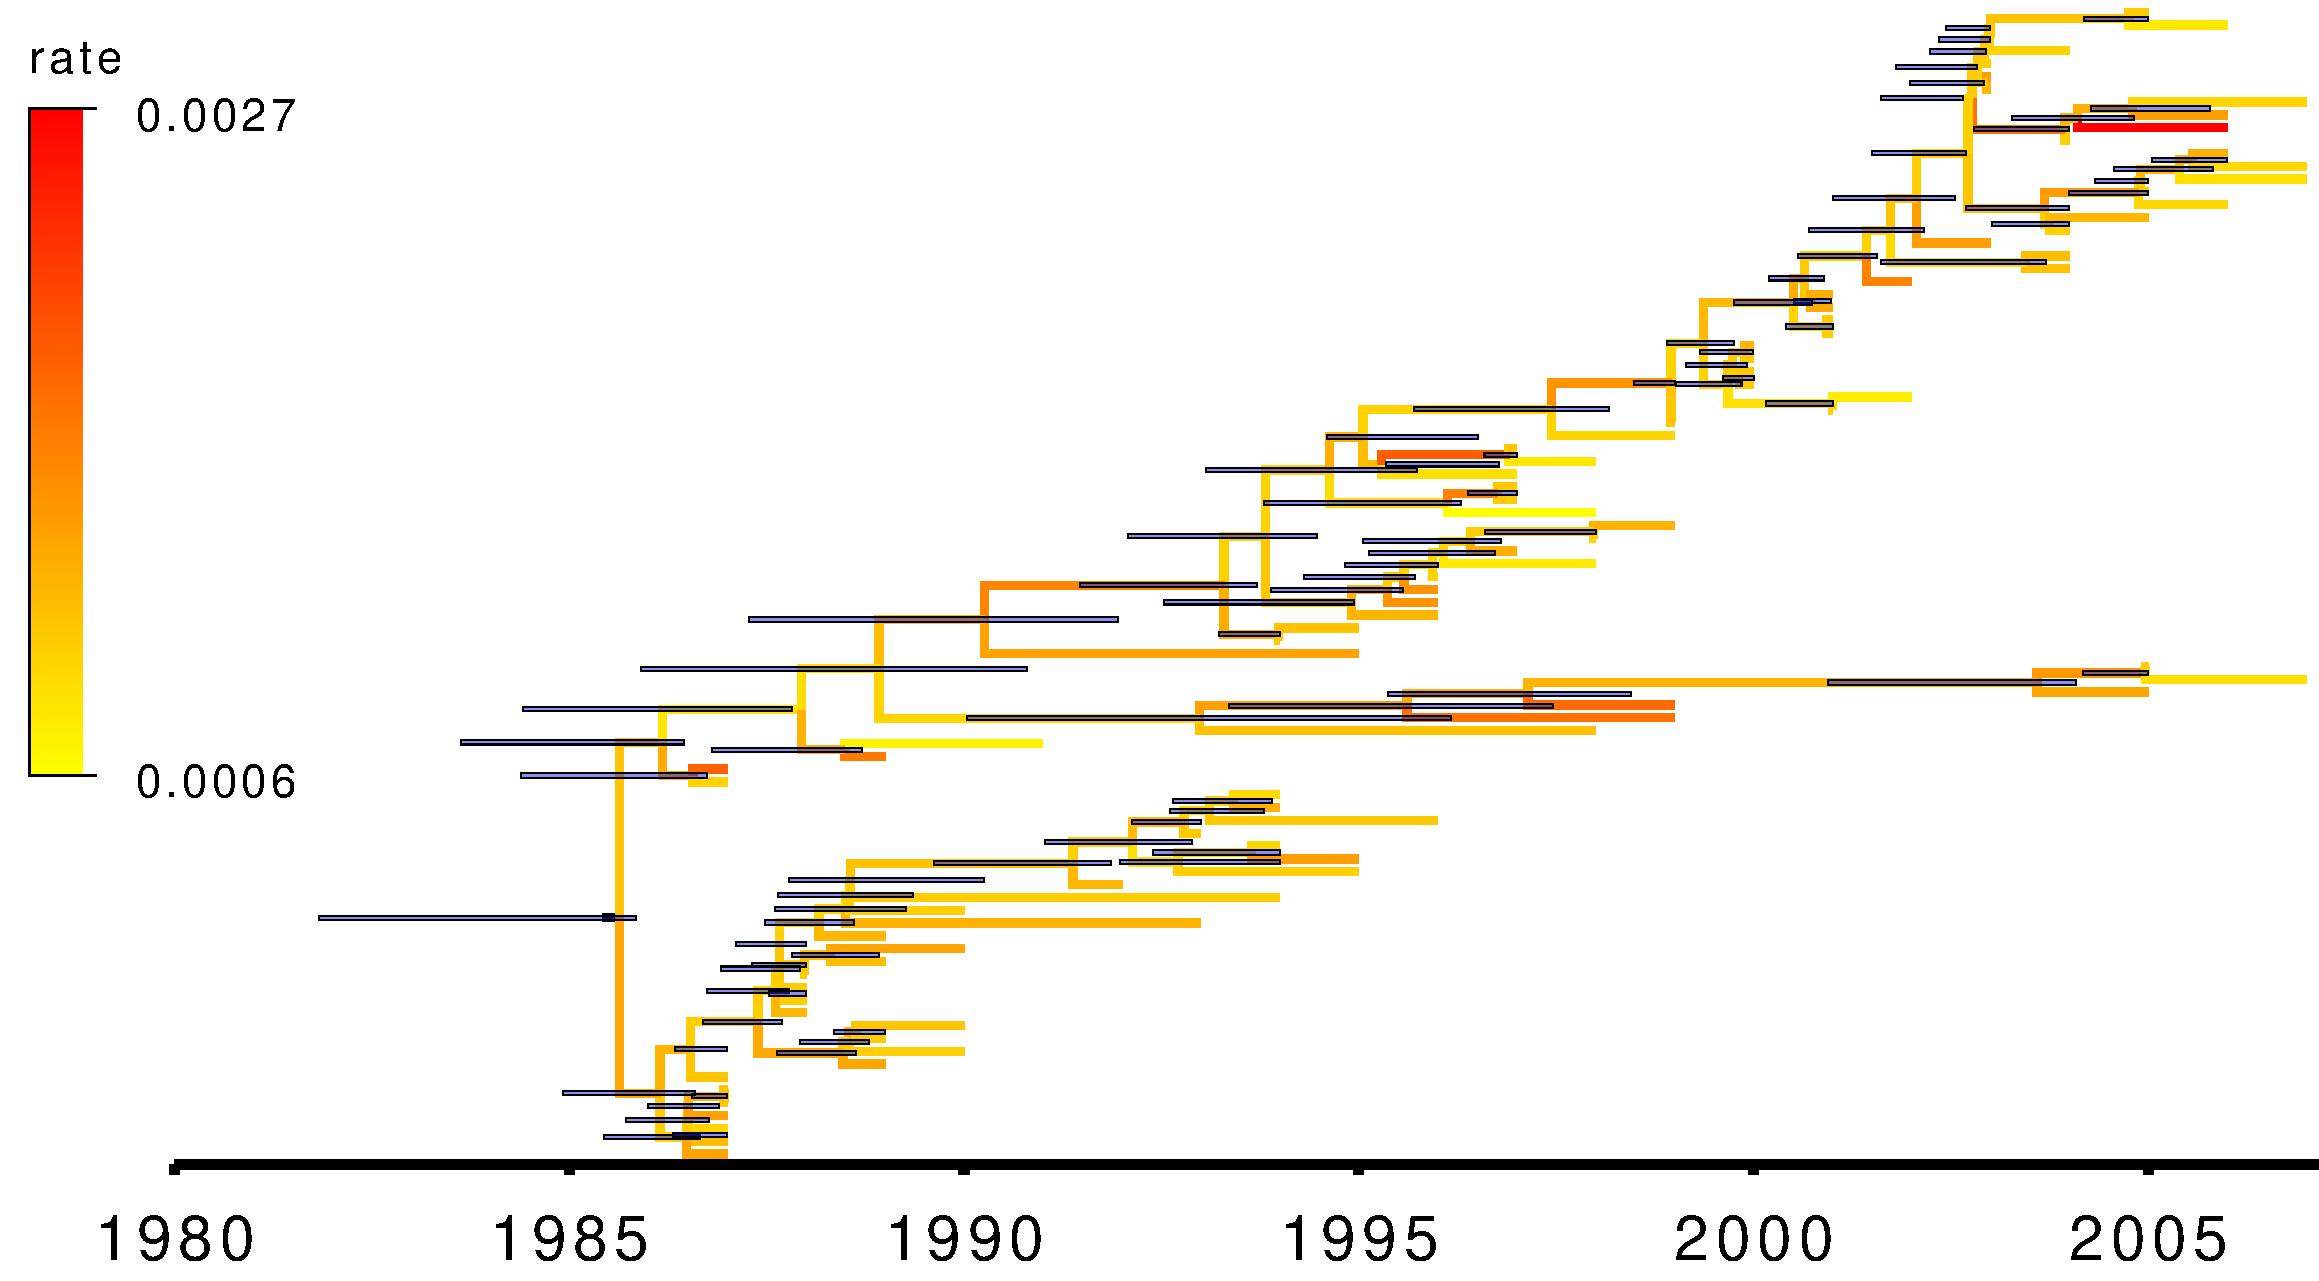
\includegraphics[scale=0.2]{\dir/figs/denv2_time_tree.pdf} 
\end{center}
 \caption[Time-calibrated phylogeny of DENV-2 strains circulating in the Americas.]{\textbf{Time-calibrated phylogeny of DENV-2 strains circulating in the Americas.}
 Phylogeny constructed using $90$~\textit{env} gene sequences from dengue virus serotype 2 (DENV-2) strains isolated in the Americas over  a large time span. 
 Branches are coloured according to their  evolutionary rates (posterior mean) and the blue horizontal bars are the 95\% highest probability density intervals for the node ages. 
 }
 \label{fig:timetree}
\end{figure}

The growing mass of available data calls for the development of more realistic evolutionary models that can in turn be used to improve phylodynamic inference, while being statistically principled and computationally tractable~\citep{Pybus2013}.
\cite{Frost2015} list eight challenges in phylodynamic inference, of which one is of special importance to the work presented here: ``how can analytical approaches keep up with advances in sequencing?''
Moreover, recent efforts have also advocated for the real-time analysis of sequence data as way of obtaining early insight into epidemic dynamics and inform intervention~\citep{Quick2016,Dudas2017,Hadfield2017}.
The combination of rapid increase in data and the necessity of timely analyses leads to an increased demand for more efficient estimation methods.

A key assumption in many phylodynamic methods is that the phylogeny is a good proxy for the~\textbf{dependence structure} of the data, even it is rarely framed in this way.
A good example of this is statistical interplay is given in~\cite{Pybus2012}, where the authors use time-calibrated phylogenies together with the sequences sampling locations and  to obtain estimates of spatial epidemiological parameters such as the velocity of the epidemic wave front and the (spatial) diffusion coefficient for the West Nile virus (WNV) epidemic in the United States of America.
\cite{Pybus2012} employ the phylogeny estimated from full WNV genomes as a~\textit{proxy} for the latent (unobserved) spatial dependence between cases and then proceed to~\textbf{condition} on the phylogeny in order to infer the epidemiological parameters.
Similarly, methods such as the continuous-time Markov chain (CTMC) phylogeography approach of~\cite{Lemey2009} rely on the estimated phylogeny -- and traits observed at the tips/leaves -- to estimate migration (transition) rates between locations.
This is a key concept in phylodynamics: even if the phylogeny is but a nuisance parameter, one needs to ensure it is estimated correctly so that inferences made conditional on the underlying dependence structure are correct.
Consequently, even if one is interested solely in epidemiological parameters, properly accommodating uncertainty about the phylogeny is crucial to principled modelling.
As I will show in the following sections, Bayesian methods provide a principled way of accounting for uncertainty about parameters and models and have proven particularly useful in phylogenetics and phylodynamics.


\section{Bayesian/Laplacian approach to inference}
\label{sec:bayesian_inference}

This thesis is fundamentally a description of how modern statistical methods can be applied to the emerging field of phylodynamics to facilitate epidemiological inference.
As such, it needs a detailed description of the underlying approach to statistical inference adopted.
In what follows I shall present a short overview of the philosophical and historical roots of the Bayesian paradigm and then move on to present the necessary technical background.

\subsection{A philosophical (and historical) digression}

In theory, Statistics can understood under two main paradigms or schools of thought: orthodox/frequentist and Bayesian/Laplacian.
The contrasts between these schools stem from fundamental disagreements on the nature and meaning of probability in modelling and interpreting reality.
Under frequentism, probabilities are understood as long run frequencies of events while under (most versions of) Bayesianism, probabilities are understood as degrees of belief~\citep{Lindley2000}.
While the two schools differ in their understanding of the meaning of probability, there is complete agreement in the~\textit{computation} of probabilities once a model has been established.
Moreover, in practice -- \textit{i.e.} real problem-solving as opposed to musing over toy problems -- there is substantial overlap and ``hybrid'' approaches often succeed~\citep{Kass2011}.

A fair and detailed comparison of these approaches is well beyond the scope of this thesis and chapter.
While preferring the Bayesian approach myself, I often find common -- short --  justifications of Bayesian inference to be wanting.
I will instead choose to gloss over important objections and assume the Bayesian paradigm for statistical inference without further justification.
I urge the reader to consult Chapter 11 of~\cite{Robert2007} for a grounded and well constructed defence of the Bayesian approach.
\cite{Jaynes2003} also offers a rather assertive argument in favour of Bayesianism.
For a grounded and modern defence of frequentism, please see~\cite{Mayo2011} and references therein.
Finally, for a modern and detailed account of~\textit{how} to do Bayesian statistics I recommend~\cite{Gelman2014b}.

The name ``Bayesian'' stems from a paper published by Thomas Bayes (1702--1761) in 1763~\citep{Bayes1763}\footnote{The attentive reader will notice that Bayes was dead by the time the paper was published. His friend Richard Price finished the paper and read it in front of the Royal Society.} on so-called ``inverse probability'', a concept emerging directly from the definition of conditional probability.
It can however be argued that Pierre Simon Laplace (1749--1827) was really the first to apply mathematically rigorous ``inverse probability'' models to scientific problems (see e.g.~\cite{Laplace1774}\footnote{An English translation is provided in~\cite{Stigler1986}.}).
It is therefore my humble opinion that we owe as much or more to Laplace as we do to Reverend Bayes for laying out the foundations of statistical thinking.
Thus a perhaps more accurate name for this approach would be Bayesian-Laplacian.
For convenience, however, I shall refer to this approach as~\textit{Bayesian} from here onwards.
 
\subsection{Bayes' rule}

Suppose one has a (probabilistic) model that describes how a random variable $\boldsymbol Y$ relates to a set of parameters $\boldsymbol\theta$ through a \textbf{likelihood} function $f(\boldsymbol Y| \boldsymbol\theta)$.
Suppose further that one observes a set of data $\boldsymbol y$.
Under the Bayesian approach, one aims to use~\textit{Bayes' rule} to construct the \textbf{posterior} distribution
\[ p(\boldsymbol\theta | \boldsymbol y) = \frac{f(\boldsymbol y| \boldsymbol\theta) \pi(\boldsymbol\theta)}{\int_{\boldsymbol\Theta}f(\boldsymbol y| \boldsymbol\theta) \pi(\boldsymbol\theta)d\boldsymbol\theta } ,\]
often written as $p(\boldsymbol\theta | \boldsymbol y) \propto f(\boldsymbol y | \boldsymbol\theta)\pi(\boldsymbol\theta)$.
This construction of the inference problem necessitates a probability measure over the parameter space, \textit{i.e.}, a \textbf{prior}, $\pi(\boldsymbol\theta)$.
In scientific applications, a common interpretation of this approach is that $\pi(\boldsymbol\theta)$ encodes our knowledge about the parameters $\boldsymbol\theta$~\textit{before} we observe the data $\boldsymbol y$ and $p(\boldsymbol\theta | \boldsymbol y)$ represents our updated beliefs/knowledge.

Two points are worth emphasising: firstly, in contrast to~\textit{maximum likelihood} and other approaches, Bayesian inference focuses on~\textit{integrating} over the likely values of the quantities of interest rather than~\textit{maximising}, that is, finding the value $\hat{\boldsymbol\theta}$ that maximises the likelihood.
Secondly, all inferences are based on the posterior; point estimates can be derived as expectations\footnote{Mathematically, expectations are integrals.} and any functionals of interest can be studied by transforming $p(\boldsymbol\theta | \boldsymbol y)$. 
The computation of posterior distributions is difficult for all but the simplest models of interest in practice.
Often, these distributions are not available analytically and must be approximated.
In Section~\ref{sec:mcmc} I present a popular method for obtaining such approximations, which will be the main focus of Chapter 2.

\subsection{Bayesian phylogenetics}
\label{sec:bayesian_phylogenetics}

While the application of Bayesian methods in phylogenetics is not without controversy~\citep{Barker2015}, this approach has enjoyed notable success in phylogenetics.
After the pioneering work of~\cite{Kuhner1995}, the mid 1990s to early 2000s saw a period of rapid development of Bayesian methods to solve phylogenetic problems~\citep{Rannala1996,Mau1997,Yang1997,Kuhner1998,Larget1999,Li2000,Suchard2001,Drummond2002}.
See~\cite{Huelsenbeck2001b} and~\cite{Holder2003} for reviews of those developments.

The main idea behind Bayesian phylogenetics is to compute a posterior distribution of the form:
\begin{equation}
 \label{eq:phylo_post_simple}
 p(T, \theta | D) \propto f(D| T, \theta)\pi(T, \theta)
\end{equation}
where $D$ is the observed data, usually an alignment of DNA sequences, $T$ is a phylogeny and $\theta$ represents parameters such as the evolutionary rate, transition/transversion rate and coalescent parameters (see below).
The likelihood is usually based on continuous-time Markov chain (CTMC) models of evolution~\citep{Hasegawa1985,Tavare1986} and be efficiently computed using a dynamic programming  procedure called ``Felsenstein's pruning algorithm''~\citep{Felsenstein1981}.
The joint prior $\pi(T, \theta)$ can be constructed in several ways, discussed in more detail below (Section~\ref{sec:coalescent_priors}) and in Appendix A.
This joint posterior can then be used to test evolutionary hypotheses, draw inference about population dynamics and obtain estimates of quantities of direct interest, such as the rate of substitution.
In many applications we are mainly interested in $\theta$, with $T$ being a nuisance parameter.
The main methodological then problem is accommodating phylogenetic uncertainty -- \textit{i.e} uncertainty about the true underlying ancestry that generated the data -- by~\textit{marginalising} over the distribution of phylogenies to obtain a distribution $p(\theta | D)$.
I shall return to the point of efficient marginalisation in Section~\ref{sec:mcmc}.

In addition to providing a principled framework for accommodating uncertainty, Bayesian phylogenetics also allows for the estimation directly interpretable  quantities, such as the posterior probability for a given clade, which are useful in assessing evolutionary hypotheses.
As mentioned above, the focus on marginalisation naturally leads to measures of uncertainty.
While authors such as~\cite{Huelsenbeck2002} have stated that Bayesian methods are also more computationally efficient\footnote{Insofar as the most popular method to approximate posterior distributions, Markov chain Monte Carlo, allows for simultaneous estimation of all quantities of interest.}, I argue that the main advantage of the Bayesian approach -- and perhaps its greatest weakness -- is the ability of the researcher to incorporate substantive expert knowledge into the analysis~\textit{via} careful construction of the prior(s).

As the field progressed and Bayesian methods became the~\textit{de facto} standard, researchers began to scrutinise the construction of prior distributions and their effects 
on inferences~\citep{Huelsenbeck2002,Yang2005,Alfaro2006}.
When little is known about the quantity of interest, researchers usually resort to ``non-informative, ignorance priors.
\cite{Seaman2012} alert on the effects of specifying such priors on model parameters as these can induce rather informative priors on quantities of interest, specially when these quantities are non-linear functions of the parameters.
A characteristic of phylogenetic models is that they tend to be rather complex and some parameters are non-linearly related.
See, for instance,~\cite{Yang1996} (and Figure 2 therein) for a discussion on the relationship between the Gamma heterogeneity parameter $\alpha$ and the transition/transversion ratio $\kappa$ under the HKY85~\citep{Hasegawa1985} model.
\cite{Rannala2012} and~\cite{Wang2014} also show that seemingly innocuous priors on the branch lengths can have rather extreme effects on the prior for tree length.


\subsection{Coalescent models as phylogenetic priors}
\label{sec:coalescent_priors}

As discussed above, performing Bayesian  inference entails assigning a probability measure over the parameter space.
One way of constructing a prior measure on the space of phylogenies is by considering the so-called~\textit{coalescent}, described in the pioneering work of~\cite{Kingman1982}.
The idea behind the coalescent is to mathematically describe the joining (coalescence) of lineages backwards in time until their common ancestor.
The main idea is to relate the effective population size $N_e$ to the probability of any two lineages joining at a certain time $t$ in the past.
For instance, in a haploid population with random mating and constant (through time) size of $N_e$, there are $2N_e$ possible coalescence points (parents) in the previous generation, which leads to there being a probability of $1/2N_e$ that any two lineages coalesce.
See below for other models of population dynamics that allow for $N_e$ to change over time.
When $N_e$ is sufficiently large, we can approximate the probability that any two lineages coalesce after time $t$ by
$$ P(t) = \frac{\exp\left( -(t-1)/2N_e\right)}{2N_e}  $$
Please see Appendix A (Section~\ref{sec:prior_maths}) for more details on the measure induced by coalescent priors on phylogenetic space.

\subsubsection{Parametric tree priors}

As seen above, the simplest model one can consider is when $N_e$ has remained constant through time, at size $N$:
$$ N_e (t) = N.$$
This population size $N$ hyper-parameter can be given a prior and estimated from the data.
This model is suitable whenever the population has remained stable over the time span of the most recent common ancestor of the samples, and provides a baseline to which more parameter-rich models can be compared.
One such example of more complex model is the exponential model, which has two parameters: the initial population size $N_0$ and the growth rate $r$.
The assumption is that population grew exponentially since the time to the most recent common ancestor (tMRCA):
$$ N_e(t) = N_0 \exp(rt), $$
which is suitable to the analysis of early viral samples from epidemics due to initial epidemic growth being approximately exponential.

\subsubsection{Non-parametric models}

These parametric models might, however, prove too inflexible in approximating population trajectories in real data.
Fortunately there are non-parametric models that allow a flexible approach to demographic modelling by constructing a piece-wise process which models population size changes between coalescent events (inter-coalescent intervals)~\citep{Pybus2000,Minin2008,Gill2012}.

The first such model I will consider here is the Skyride model~\citep{Minin2008}, which improves on previous semi-parametric models~\citep{Pybus2000} of piece-wise population size change by (i) assuming population size changes smoothly over time and (ii) places a smooth Gaussian process prior on the population sizes.
Skyride operates on inter-coalescent intervals, i.e., intervals of time between coalescent events (represented by internal nodes in a phylogeny, see Appendix A for a rigorous exposition).
For a phylogeny with $n$ tips/leaves, let $\boldsymbol s = ( \boldsymbol s_2, \ldots, \boldsymbol s_n )$ be the inter-coalescent intervals.
If sampling is heterochronous, sampling times further divide inter-coalescent intervals in sub-intervals, i.e., $\boldsymbol s_k = (s_{k0}, \ldots, s_{kj_{k}} ) $.
If we denote the population sizes by $\boldsymbol \theta = ( \theta_2, \ldots, \theta_n )$, the likelihood becomes 
$$ Pr(\boldsymbol s | \boldsymbol \theta) = \prod_{k = 2}^n Pr(s_k | \theta_k), $$
with
$$ Pr(s_k | \theta_k) = \frac{n_{k0} (n_{k0} - 1)}{2\theta_k} \exp\left( - \sum_{j=0}^{j_{k}} \frac{ n_{kj} (n_{kj} - 1)s_{kj} }{2\theta_k}\right). $$
If we make the convenient transformation $\gamma_k = \log(\theta_k), k = 2, \ldots, n $, we can then place the Gaussian Markov random field (GMRF) prior on $\boldsymbol \gamma $:
$$ Pr(\boldsymbol \gamma | \tau ) \propto \tau^{(n-2)/2} \exp\left(- \frac{\tau}{2} \sum_{k = 2}^{n-1} \frac{(\gamma_{k + 1} -\gamma_k)^2}{\delta_k} \right), $$
where $\delta_k$ is the (1d) distance between intervals and $\tau$ is the precision parameter associated with the smoothing.
For details please see~\cite{Minin2008}.

The second model I will consider is the Skygrid model, an extension of the Skyride that allows for multiple loci.
While in Skyride the estimated trajectory changes at coalescent times, in Skygrid changes occur at pre-specified fixed points in (real) time.
This allows population sizes to be estimated for multiple genealogies at once, e.g., when several genes are under analyses and have different genealogies.
The researcher must select the number $M$ of grid points to be used and a cutoff $K$ in calendar time.
The cutoff $ K $ is crucial to the Skygrid analysis, as it is the last point at which population sizes change and hence should be chosen commensurate with the age of the root.
As with Skyride, the smoothness of the Skygrid prior is controlled by a precision parameter $\tau$.
The Skygrid model presents better statistical properties and is more general, which has led to it superseding Skyride in recent years.
These models are parameter-rich and their use is preferable when the data are strongly informative about population history.
More recent developments allow for the inclusion of (time) covariates to inform the population sizes in Skygrid~\citep{Gill2016}, which not only promises to help with~\textit{understanding} population dynamics but also offers a way of introducing information to inform the non-parametric prior and regularise inference.


Historically, in addition to being used to construct prior distributions these models have been used directly to investigate how distinct patterns of coalescence and genetic diversity relate to population epidemiological processes, specially for viruses~\citep{Rodrigo1999,Pybus2000,Pybus2009}.

\subsubsection{Other priors}

While the coalescent offers a flexible framework for modelling the population dynamics from genealogies, it also relies on restrictive assumptions.
For instance, the coalescent assumes that the fraction of sampled individuals (number of taxa, $n$) is a negligible fraction of total population.
With the rapid increase in the number of sequences, it is quite possible that an epidemic could be sampled to 5\% or more of its total cases, therefore rendering this assumption problematic.
To address this and also allow for more explicit models of epidemic dynamics, several models based on birth-death processes,~\cite{Volz2009},~\cite{Rasmussen2011} and~\cite{Stadler2011} have developed approaches that incorporate other population models such the Yule process and epidemic models such as the Susceptible-Infected-Removed (SIR) model.
Similarly to the coalescent, these models too can be used as prior measures for phylogenies, and in addition be used to estimate parameters of interest such as $R_0$.

\section{Markov chain Monte Carlo}
\label{sec:mcmc}

Since the phylogenetic posterior~(\ref{eq:phylo_post_simple}) is not available in closed-form even for the simplest models, it must be numerically approximated.
In the following sections I introduce the necessary mathematical background for Markov chain Monte Carlo (MCMC), which I will base mostly on~\cite{Geyer2011}.
For ease of exposition, whenever a choice is to be made between a discrete and a continuous setting I shall assume the latter -- as shown in Appendix A, phylogenetic space has both discrete and continuous components.

Suppose one aims to sample from a distribution\footnote{I will assume the target is either normalised or can be normalised,~\textit{i.e.}, $ 0 < \int_{\mathcal{X}} \pi_d(x) <\infty$. } $\pi(\cdot)$ defined on a sample space $\mathcal{X}$, with density $\pi_d$ such that 
\[ \pi(U) = \frac{\int_{U} \pi_d(x)dx }{\int_{\mathcal{X}} \pi_d(x)dx}. \]
One reason to obtain samples from $\pi(\cdot)$ is to compute expectations of functionals $f :\mathcal{X} \to \mathbb{R}$ such that
\[ \pi(f) = \mathbb{E}_{\pi} [f(X)] = \int_{\mathcal{X}} f(x) \pi(x) dx. \] 
Classic Monte Carlo theory says that, under some mild regularity conditions, if one obtains a sample of i.i.d. random variables $\boldsymbol Z = \{ Z^{(1)}, Z^{(2)}, \ldots, Z^{(N)} \} \sim \pi(\cdot)$, then
\[ \hat{\pi}(f) = N^{-1}\sum_{i=1}^N f(Z^{(i)}), \]
is an unbiased estimate of $\pi(f)$.
Moreover, the standard deviation of $\hat{\pi(f)}$ is $\mathcal{O}(\frac{1}{\sqrt{N}})$, meaning we can make the estimate as precise as desired by increasing the number of samples $N$.
Obtaining $\boldsymbol Z$ directly, however, might be impractical.
Instead, Markov chain Monte Carlo (MCMC) is a technique to draw samples by constructing a Markov chain $\{X_i\}$ on $\mathcal{X}$ that has $\pi(\cdot)$ as its~\textit{limiting} (or stationary) distribution. 
More formally, we want to construct $\{X_i\}$ with transition probabilities $P(x, dy)$ such that
\[ \pi(dy) = \int_{\mathcal{X}} \pi(dx) P(x, dy)  \]
for all $x,y \in \mathcal{X}$.
If we are able to draw samples from this Markov chain, then for a sufficiently large number of samples we will obtain a collection of random variables that are approximately drawn from $\pi(\cdot)$.

We are still however left with the task of finding an appropriate $P(x, dy)$.
One useful simplifying assumption usually made is that $P(x, dy)$ is~\textit{reversible}:
\[ \pi(dx) P(x, dy) = \pi(dy) P(y, dx) .\]
This condition is also known as~\textbf{detailed balance} and ensures $\{X_i\}$ has $\pi(\cdot)$ as its stationary (limiting) distribution.
One of the simplest ways of constructing a reversible Markov is the so-called Metropolis-Hastings algorithm, described in Section~\ref{sec:MH}. %TODO: next section (if doesn't change).

\subsection{Metropolis-Hastings}
\label{sec:MH}

Let $q_\sigma(x, y)$ be a~\textit{candidate-generating} density with indexing parameter%\footnote{The reasons for the inclusion of this parameter shall become clearer in Section~\ref{sec:practical}.}
$\sigma$ such that $\int_{\mathcal{X}} q_\sigma(x, v) dv = 1 \: \forall x \in \mathcal{X}$. 
Now consider a Markov chain $Q_\sigma(x, \cdot)$ such that $Q_\sigma(x, y) \propto q_\sigma(x, y) dy$.
The so-called Metropolis-Hastings (MH) algorithm~\citep{Metropolis1953,Hastings1970} consists of constructing a Markov chain with acceptance probability
\begin{equation}
 \label{eq:acceptance}
 \alpha_\sigma(x, y) = min \left[1, \frac{\pi_d(y) q_\sigma(y, x)}{\pi_d(x) q_\sigma(x, y)} \right],
\end{equation}
with $\alpha_\sigma(x, y) = 1$ if $\pi_d(x) q_\sigma(x, y)$.
The quantity $q_\sigma(y, x)/ q_\sigma(x, y)$ is called the ``Hastings ratio'' and acts as a correction factor to ensure we sample from the desired target (see below).

Computationally, MH can be described as generating samples $\boldsymbol Z$ as follows:
\begin{enumerate}
 \setcounter{enumi}{-1}
 \item Pick some $Z^{(0)} \in \mathcal{X}$;
 \item Given $Z^{(n)}$, generate a \textit{proposal} $Y^{(n + 1)} \sim Q_\sigma(Z^{(n)}, \cdot)$;
 \item Sample $u \sim \text{Uniform}(0, 1)$;
 \item If $\alpha_\sigma(Z^{(n)},  Y^{(n + 1)}) > u$, set $Z^{(n + 1)} = Y^{(n + 1)}$, otherwise $Z^{(n + 1)} = Z^{(n)}$ ;
 \item Repeat steps 1 through 3 until $M$ samples are obtained.
\end{enumerate}
This can be shown to correctly sample from $\pi(\cdot)$ for appropriately chosen $q_\sigma(\cdot, \cdot)$ (see below) and is straightforward to implement on a computer.
The MH algorithm is a very popular workhorse of MCMC, much due to its simplicity of implementation.
Good introductions can be found in~\cite{Chib1995} and~\cite{Robert2015}.

While the MH algorithm is by far the most popular algorithm in MCMC, it is by no means the only one.
A very popular method is the Gibbs sampler~\citep{Geman1984}, an algorithm whereby samples $\pi(\cdot)$ are drawn from a series of conditional distributions, which can be quite useful when sampling Bayesian posterior distributions based on conjugate priors.
When sampling from spaces with varying dimension, the so-called ``Reversible-jump'' MCMC of~\cite{Green1995} has enjoyed great success.
Perhaps not surprisingly, many of these algorithms are special instances of a more general sampling procedure, as shown by~\cite{Keith2004}.
A common criticism of MH is the fact that the transitions (step 3 above) do not take into account the structure of the target, often leading to random-walk behaviour.
Algorithms such as the Metropolis-adjusted Langevin algorithm (MALA)~\citep{Roberts1998} and Hamiltonian (Hybrid) Monte Carlo (HMC)~\citep{Duane1987,Neal2011} exploit the structure of the target -- usually in the form of gradients -- to perform guided transitions and increase efficiency.
I discuss this point further in Chapter 6.

\subsection{Transition kernels}
\label{sec:kernels}

Successful exploration of the target distribution depends crucially on the choice of $Q_\sigma(\cdot, \cdot)$.
In particular, the~\textbf{transition kernel}
\begin{equation}
 \label{eq:transition_kernel}
 \kappa_\sigma(x, dy) = q_\sigma(x, y) \alpha_\sigma(x,y)dy  + \left[1 - \int_{\mathcal{X}} q_\sigma(x, y) \alpha_\sigma(x,y)dy \right]\delta_x(dy),
\end{equation}
where $\delta_x(u) = 1$ if $x \in u$ and $0$ otherwise, needs to be constructed carefully to ensure correct and efficient sampling.
Here I briefly discuss some of the aspects, both practical and theoretical, involved in designing effective transition kernels.
Further discussion of transition kernels in MCMC for Bayesian phylogenetics can be found in Chapter 2.

The first point to notice is that for complex parameter spaces, the construction of the proposal might be quite complicated, and the the density  $q_\sigma(\cdot, \cdot)$ might be hard to compute.
\citep{Green2003} proposes a constructive method for computing the acceptance ratio that simplifies calculations, specially when considering varying-dimension problems.
Denote the current state of the chain is $x$ and the proposed (candidate) state is $x^\prime$.
The main idea is to sample a set of auxiliary random variables $\boldsymbol u \in \boldsymbol U$ from a distribution $g(\cdot)$ and then apply a transformation $h : \mathcal{X} \times \boldsymbol U \to \mathcal{X} $ such that $x^\prime = h(x, \boldsymbol u)$.
To obtain $x$ from $x^\prime$ the procedure is to generate a set $\boldsymbol u^\prime \in \boldsymbol U$ from a (potentially different) distribution $g^\prime(\cdot)$ and apply a transform $h^\prime : \mathcal{X} \times \boldsymbol U \to \mathcal{X}$ to get $x = h^\prime(x^\prime, \boldsymbol u^\prime)$.
The acceptance probability can then be written as 
\[
 \alpha^\star_\sigma(x, y) = min \left[1, \frac{\pi_d(y) g_d^\prime(\boldsymbol u^\prime)}{\pi_d(x) g_d(\boldsymbol u)} |J| \right],
\]
with $J = \text{det} \left[\frac{\partial (x^\prime, \boldsymbol u^\prime) }{\partial (x, \boldsymbol u)} \right]$.
See~\cite{Holder2005} for an application of this technique in Bayesian phylogenetics, where it was used to correct an error in the original derivation of the \verb|LOCAL| transition kernel~\citep{Larget1999}.


\subsection{Some considerations on MCMC}
\label{sec:practical}

In practice, there are many details that determine the effectiveness of MCMC as a numerical method.
One of the key challenges in efficiently computing an approximation of the target is the boldness of the proposing mechanism: propose extreme (bold) values and the candidate is likely to be rejected, making the chain be stuck for long periods; propose conservatively and the candidate is likely to be accepted but the chain will seldom move away from the current state, leading to poor exploration.
It is therefore desirable to construct the candidate generating density so as to strike the best balance between bold and conservative proposals, a problem called optimal scaling~\citep{Roberts1998,Roberts2001}.
\cite{Gelman1996} suggest that under some regularity conditions on the target $\pi(\cdot)$, an acceptance probability of $0.234$ when the dimension of $\mathcal{X}$ is large enough will produce optimal sampling when compared with independent samples from $\pi(\cdot)$. 
More modern algorithms are~\textbf{adaptive}, meaning the transition kernel indexing parameter $\sigma$ can be ``tuned'' using the previous history of the chain to achieve the optimal acceptance probability~\citep{Haario2001}.

Another issue that has received much attention in the literature is determining whether $\{X_i\}$ has~\textit{converged in distribution} to $\pi(\cdot)$.
See~\cite{Robert2004} and~\cite{Meyn2012} for the technical details and Chapter 3 for a review on (statistical) tools to assess convergence.
Related to the issue of convergence is ascertaining that the effect of the initial state $Z^{(0)}$ is negligible.
In actual practice, approximations to functionals are usually done considering only samples after a \textbf{warm-up} (burn-in) number of iterations $W$,~\textit{i.e.}, $ \hat{\pi}(f) = (M - W)^{-1}\sum_{i = W + 1}^{W + M} f(Z^{(i)})$ (see Chapter 3).
We are usually interested on~\textbf{mixing}, that is, how well the Markov chain explores the target distribution.
Since the samples obtained by MCMC are fundamentally correlated, we can measure its~\textit{efficiency} by estimating how many independent samples from $\pi(\cdot)$ were produced.
This quantity is called the~\textbf{effective sample size} (ESS) and I provide definitions and discussion in Chapter 3.
In short, the higher the closer the ESS is to the chain length $M$\footnote{It is technically possible to have ESS larger than $M$ when using over-relaxation techniques, but this is a fringe case.}, the more efficient is MCMC in approximating $\pi(\cdot)$.

In addition to efficiency it is important to ensure comprehensive exploration of the target distribution.
In order for samples obtained with MCMC to be of any practical use, they need to represent the~\textbf{typical set} of the target distribution.
Intuitively, this is to be understood as exploring the ``bulk'' of the distribution, where most of its mass lies.
More formally, the typical set can be defined as $\boldsymbol S_\epsilon \in \mathcal{X}$ such that for all sequences $\boldsymbol X = \{X_1, X_2, \ldots, X_n \} \in \boldsymbol S_\epsilon$
\[ 2^{-n\left(H_\pi  + \epsilon\right)} \leq \pi(\boldsymbol X ) \leq 2^{-n\left(H_\pi -\epsilon\right)} \]
holds, where $H_\pi = \mathbb{E}_\pi[\log_2(x)]$ is the entropy of $\pi(\cdot)$. 
In practice we cannot know for sure whether our chain has explored the typical set.
Even, if our algorithm is correctly constructed and our efficiency measures suggest satisfactory sampling, it might be the case that our chain is stuck at a mode, for instance, and not sampling the whole space.
For most target distributions of interest in practice, the issue of determining the typical set remains an open problem.

Contrary to what is routinely suggested in the literature, MCMC is not a Bayesian method.
Rather, MCMC is a computational method for approximating integrals and is completely agnostic about what is being computed.
As a counter-example to the claim the MCMC is ``Bayesian'' in any way, I offer~\cite{Geyer1991} and~\cite{Kuhner1998}, who employ MCMC for maximum likelihood estimation\footnote{See also~\url{http://users.stat.umn.edu/~geyer/mcmc/diag.html} -- also cited in Chapter 3 -- for the precious quote ``[MCMC] isn't even statistics, it is a tool.''. Terms such as ``Bayesian MCMC'' make no sense whatsoever. }.
Moreover, MCMC is not the only tool to compute integrals and approximate distributions; rejection sampling~\citep{Casella2004} and importance sampling~\citep{Rubinstein2016} are examples of techniques that do not involve the construction of Markov chains.

\section{Software}
\label{sec:software}

In the course of my doctoral work I have written a fair amount of computer programs (scripts) to perform several custom analyses as well as to automate data wrangling and processing tasks.
In this short section I detail some of the software I have used in my research and acknowledge the efforts of the many programmers who developed these tools without which my work would not have been possible.
The first point to notice is that most (if not all) software I have used was open source software, that is, software for which the source code is released under a licence that allows the end user to study, change, and distribute the software to anyone and for any purpose~\citep{Laurent2004}.
This is important insofar as it allows one to see what is ``under the hood'', the inner workings of the software under use, a crucial aspect of ensuring scientific correctness~\citep{Darriba2018}.
Throughout my PhD I have used a GNU/Linux desktop (and server) system, which sports a host of useful tools that were crucial for my research.
The first of these tools is the bash shell, which allowed me to script many otherwise tedious and error-prone tasks.
A second tool that I made extensive use of was \verb|GNU Parallel|~\citep{Tange2011}, which allows executing jobs in parallel and hence exploit multi-core architectures in most modern personal computers and servers.

Most of the programs I wrote for my research were written in the R statistical computing language~\citep{R2017}, using the open source integrated development environment (IDE) Rstudio~\citep{Rstudio2015}.
R offers an enormous variety of user-contributed packages which greatly expand the capabilities of the base distribution. 
I have used the \textbf{ape}~\citep{Paradis2004},~\textbf{parallel}~\citep{R2017},~\textbf{ggplot2}~\citep{Wickham2009},~\textbf{viridis}~\citep{Garnier2018} and~\textbf{data.table}~\citep{Dowle2017} packages repeatedly across several projects.
This list is by no means exhaustive; please see the individual chapters for more details on the R packages (and other software) I have used in each of the projects.
BEAST (see below) is written in the cross-platform JAVA language (\url{https://java.com/}) and I have used the Eclipse IDE (\url{https://www.eclipse.org/ide/}) to aid both code reading and minor development.
Finally, I would like to mention that I have made extensive usage of the excellent code hosting service GitHub (\url{https://github.com/}) and the associated version-control system, \verb|git|.
This thesis was written using the open-source typesetting language \LaTeX and its source code is hosted at~\url{https://github.com/maxbiostat/PhD_Thesis}.

\subsubsection{BEAST}
\label{sec:beast}

The software package BEAST, short for \textbf{B}ayesian \textbf{E}volutionary \textbf{A}nalysis by \textbf{S}ampling \textbf{T}rees\citep{Drummond2007,Drummond2012} is a central focus of this thesis.
BEAST is specially designed for the estimation of rooted phylogenies, with a heavy focus on time-calibrated phylogenies.
It offers a large number of tree priors (coalescent- and non coalescent-based models) as well as specialised computational machinery for the construction and estimation of discrete and continuous phylogeographic models~\citep{Lemey2009,Lemey2010,Pybus2012,Dudas2017}.
The interested reader is referred to the on-line documentation (\url{http://beast.community/}) for more information.

With regard to MCMC, BEAST uses Metropolis-Hastings as its main algorithm, while specialised samplers do exist for some model components.
For example  a Gibbs sampler is used to efficiently sample the quantities in the Skygrid model described above.
In BEAST~\textit{parlance}, transition kernels are called~\textbf{operators} and I shall employ the terms interchangeably. 
BEAST employs adaptive MCMC, meaning that it tunes the scale of its operators to achieve a target acceptance probability -- currently $0.234$ for most operators.
It is important to notice, however, that not all operators in BEAST can be adjusted in this way, and are therefore called ``non-tunable'', in contrast to the ``tunable'' ones.

The kernels described in Chapter 2 were implemented in BEAST\footnote{I would like to explicitly acknowledge Andrew Rambaut's extensive help with understanding BEAST and its inner workings, as well as implementing many of the ideas explored in this thesis, for which I am very grateful.} and the visualisations in Chapter 3 would not have been possible without specialised classes in the BEAST code base (see Section~\ref{sec:accommodating} therein).
Moreover, BEAST output was also important in the analyses I present in Chapters 4 and 5, where I sought to combine phylodynamic data from BEAST analyses with epidemiological information.

\section{Goals}
\label{sec:goals}

Since its emergence in the later half of the 2000s, phylodynamics has grown into a powerful tool in the study of pathogen dynamics.
However, as many authors note~\citep{Volz2013,Pybus2013} note, there is an ever growing gap between data accumulation and the methodological apparatus to analyse and integrate this data.

This PhD thesis is attempt at plugging that gap, and has two main axes: the development of more efficient transition kernels and visualisations for MCMC in phylogenetic space and the application of state-of-the-art statistical methods to address phylodynamic/epidemiological questions.
In Chapters 2 and 3 I outline a proposal for new transition kernels (operators) and address the adaptation of existing convergence diagnostics to large, time-calibrated phylogenies.
Chapters 4 and 5 showcase how one can combine modern statistical tools and phylogenetic/phylodynamic data to explore the evolutionary and epidemiological dynamics of pathogens such as Ebola virus.
In chapter 6 I discuss the overall impact of the findings in this thesis and how I see the field moving forward.

% \bibliography{/home/max/Dropbox/PHD/THESIS/bibliography/lmcarvalho_PhD_Thesis}